\documentclass[a4paper,12pt]{article}
\usepackage{HomeWorkTemplate}
\usepackage{circuitikz}
\usepackage[shortlabels]{enumitem}
\usepackage{float}
\usepackage{hyperref}
\usepackage{tikz}
\usepackage{amsmath}
\usepackage{amssymb}
\usepackage{tcolorbox}
\usepackage{xepersian}
\settextfont{XB Niloofar}
\usetikzlibrary{arrows,automata}
\usetikzlibrary{circuits.logic.US}
\usepackage{changepage}
\newcounter{problemcounter}
\newcounter{subproblemcounter}
\setcounter{problemcounter}{1}
\setcounter{subproblemcounter}{1}
\newcommand{\problem}[1]
{
	\subsection*{
		پرسش
		\arabic{problemcounter} 
		\stepcounter{problemcounter}
		\setcounter{subproblemcounter}{1}
		#1
	}
}
\newcommand{\subproblem}{
	\textbf{\harfi{subproblemcounter})}\stepcounter{subproblemcounter}
}


\begin{document}
\handout
{آز طراحی سیستم‌های دیجیتال}
{دکتر سیاوش بیات سرمدی}
{نیم‌سال اول 1400\lr{-}1401}
{اطلاعیه}
{پرهام چاوشیان}
{98100118}
 {گزارش آزمایش چهارم}
{خانم زینب رشیدی}
برای پیاده‌سازی پشته، از یک حافظه کمک گرفته‌ایم. این حافظه 10 خانه دارد و هر خانه آن نیز 5 بیتی است. همچنین یک اشاره‌گر داریم که پایین‌ترین خانه خالی را نشان ‌می‌دهد. با لبه پایین رونده $RstN$ استک خالی می‌شود. مطابق با دستور کار، زمانی که استک خالی باشد، سیگنال $Empty$ مقدار صفر می‌گیرد و همچنین زمانی که پر باشد، مقدار 1 می‌گیرد. زمانی که فرمان $Push$ بیاید، اگر استک پرنباشد، ورودی را درحافظه قرار داده و اشاره‌گر را یک خانه بالا می‌بریم. زمانی که فرمان $Pop$ بیاید و استک خالی نباشد، اشاره‌گر را یک خانه پایین برده و عدد را در خروجی قرار می‌دهد.\\
نتایج شبیه‌سازی نیز در ادامه آمده است (در صورت نیاز تصاویر به طور جداگانه نیز پیوست شده اند):
\begin{figure}[H]
 \centering
  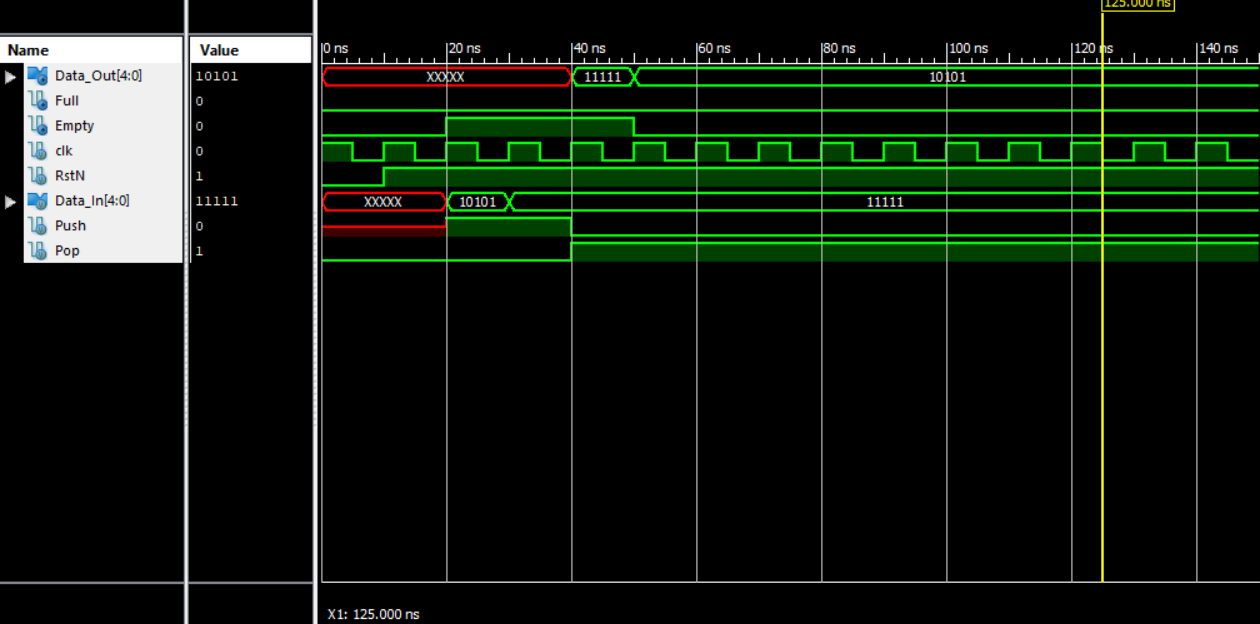
\includegraphics[width=0.8\linewidth]{s1}
\end{figure}
\end{document}